\section{Numerical specialties}
The simulation of the real time evolution is going to take some time. Since we want to simulate different parameters, we are going to have to run this simulation over and over again.
In order to speed up this procedure, we wrote GitHub automations.
Those use multiple Ubuntu instances on GitHub servers and therefore can simulate a lot of different parameters in parallel.
This speeds up the simulation time.

\section{Entanglement}
At first we are going to consider the time evolution of the on-site entanglement entropy.
Plots for $g=\num{0.2}$ and $g=\num{2}$ can be found int \autoref{fig:day2_entanglement}.
In both cases we can see a similar behavior.
We obtain a cone shaped evolution.
We will consider the reflection on the boundary for $g=\num{2}$ in the next part.
This corresponds to an overall increasing entanglement entropy.

\begin{figure}[htbp]
    \centering
    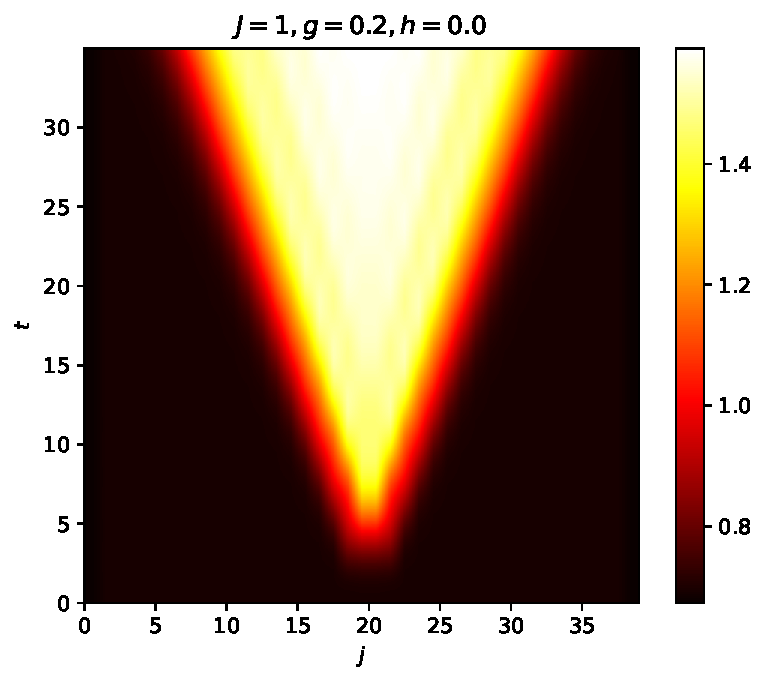
\includegraphics[width=0.49\textwidth]{day2_entanglement_L=40_g=0.2_h=0.0.pdf}
    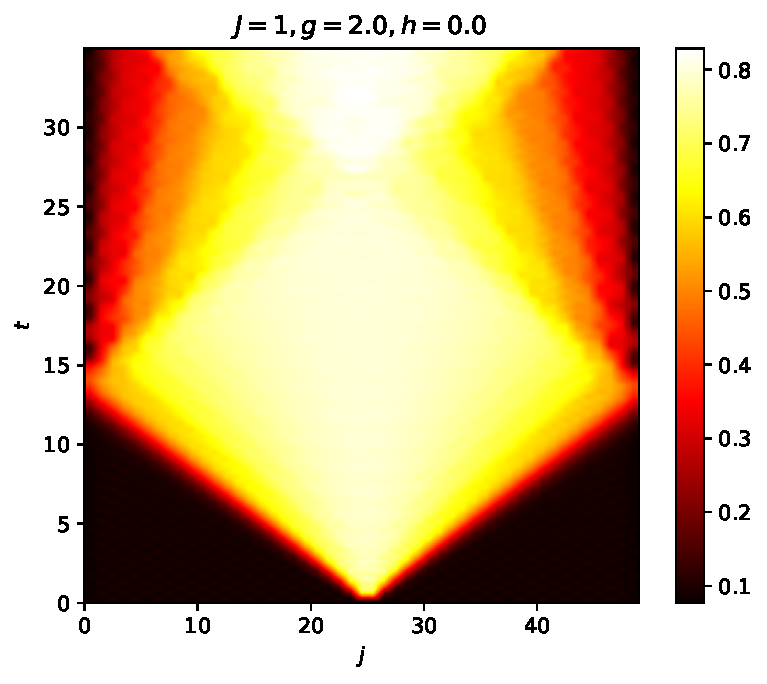
\includegraphics[width=0.49\textwidth]{day2_entanglement_L=50_g=2.0_h=0.0.pdf}
    \caption{Time evolution of the entanglement entropy of the Ising chain for different system parameters.}
    \label{fig:day2_entanglement}
\end{figure}


Having a basically vanishing entanglement entropy at the start makes a lot of sense.
At time $t=0$ we are in the ground state of the Ising model.
% This is either the ferromagnetic or paramagnetic phase.
We use a MPS approach to simulate this system.
This approach is based on the fact of having quickly decreasing Schmidt coefficients, since we cut off those off at some point.
Therefore having low entanglement at the start is in correspondence with our requirements for a stable numerical simulation.

If we let the system evolve, the sites will couple to each other, because of correlations between them.
This leads to an increased entanglement, as can be seen in the plots.


% -----------------
% \begin{figure}[htbp]
%     \centering
%     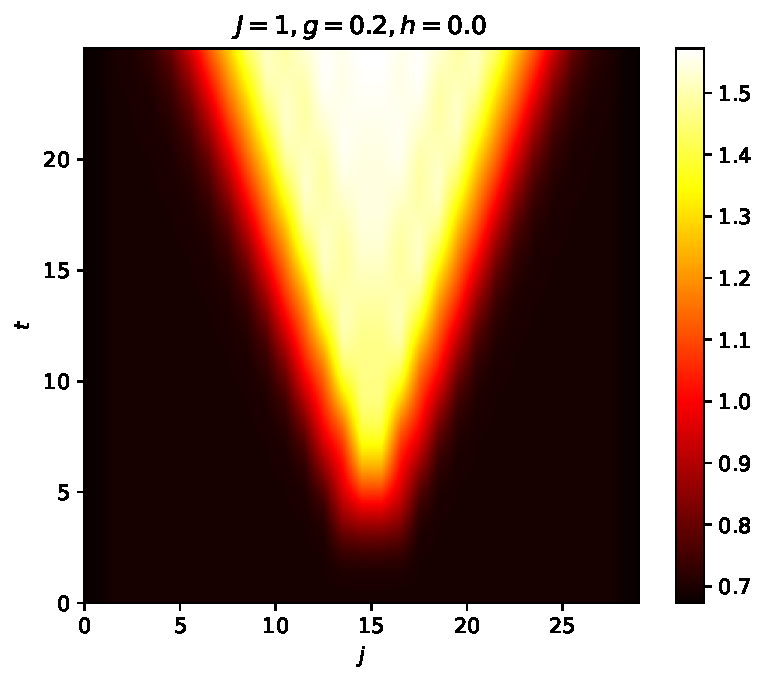
\includegraphics[width=0.7\textwidth]{day2_entanglement_L=30_g=0.2_h=0.0.pdf}
%     \caption{}
% \end{figure}

% \begin{figure}[htbp]
%     \centering
%     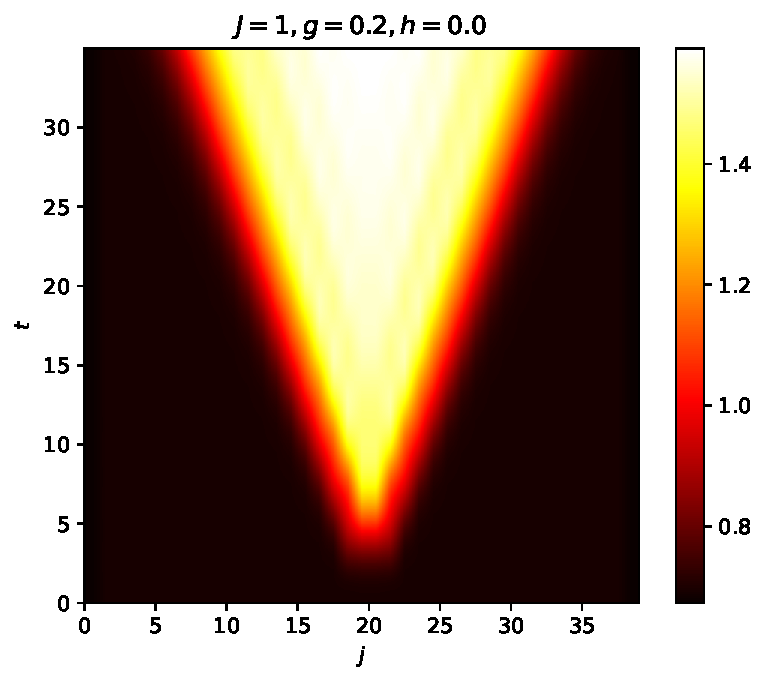
\includegraphics[width=0.7\textwidth]{day2_entanglement_L=40_g=0.2_h=0.0.pdf}
%     \caption{}
% \end{figure}

% % not generated yet
% % \begin{figure}[htbp]
% %     \centering
% %     \includegraphics[width=0.7\textwidth]{day2_entanglement_L=50_g=0.2_h=0.0.pdf}
% %     \caption{Time evolution of the entanglement entropy in the }
% % \end{figure}

% \begin{figure}[htbp]
%     \centering
%     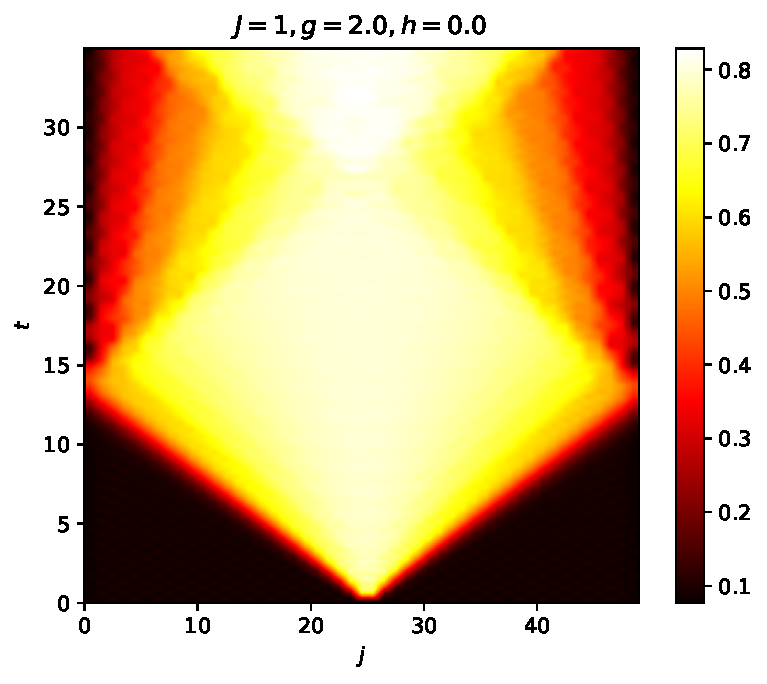
\includegraphics[width=0.7\textwidth]{day2_entanglement_L=50_g=2.0_h=0.0.pdf}
%     \caption{}
% \end{figure}

% \begin{figure}[htbp]
%         \centering
%         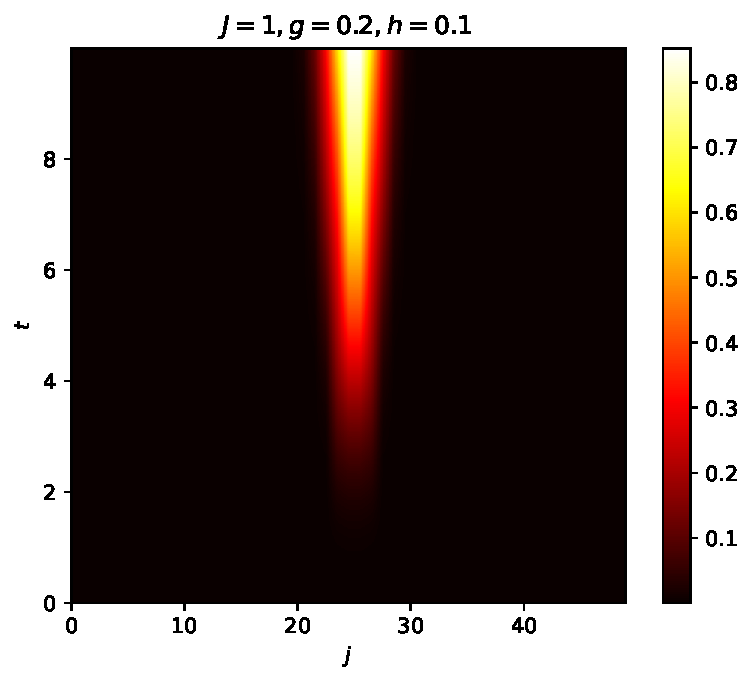
\includegraphics[width=0.7\textwidth]{day2_entanglement_L=50_g=0.2_h=0.1.pdf}
%         \caption{Time evolution of the entanglement entropy in the }
% \end{figure}


% \newpage
\section{Correlation}
We now take a closer look at the correlations of the system.
Here we can also see, that we start of with very localized correlations around our reference point at $L/2$.
As the system evolves, those correlations spread out to the sides.
We can see this in the form of \enquote{strings} rising to the top of the plot.

Those correlations also cause the increase of entanglement and therefore our observations are consistent within themselves.

Physically speaking, we insert an excitation at the spin at position $L/2$ in the system.
This excitation can freely propagate and will do so.
This can be seen by the fact, that the correlations grow out over time.
In the $g=2$ plot we can see something interesting.
In this case, the excitation bounces off the wall.
This is obviously not what we would expect in the real world, since this is only caused by the fact that we are limited to finite size systems.
Nevertheless it is still really interesting to see, that the correlation does not vanish in noise, but we can still clearly see the reflected propagation.

\begin{figure}[htbp]
    \centering
    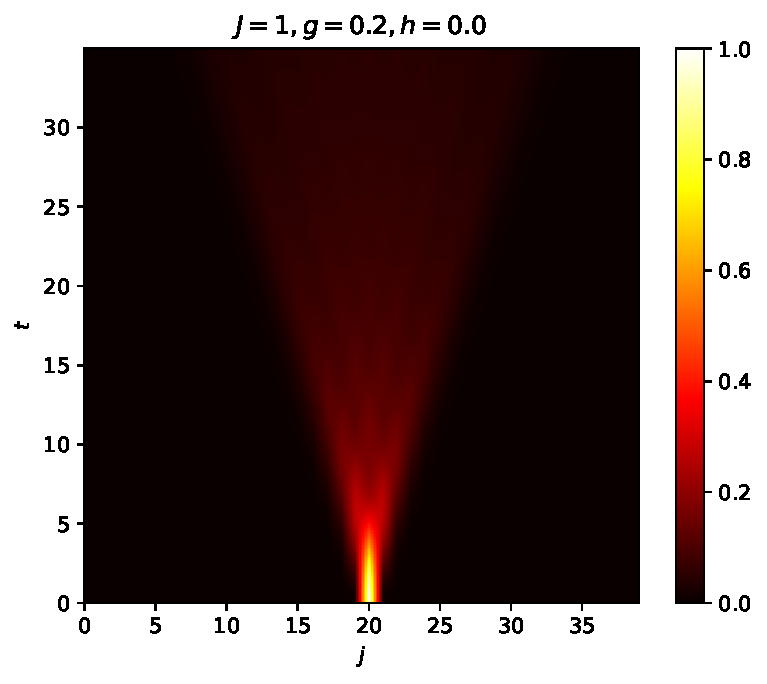
\includegraphics[width=0.49\textwidth]{day2_correlation_g=0.2_L=40_h=0.0.pdf}
    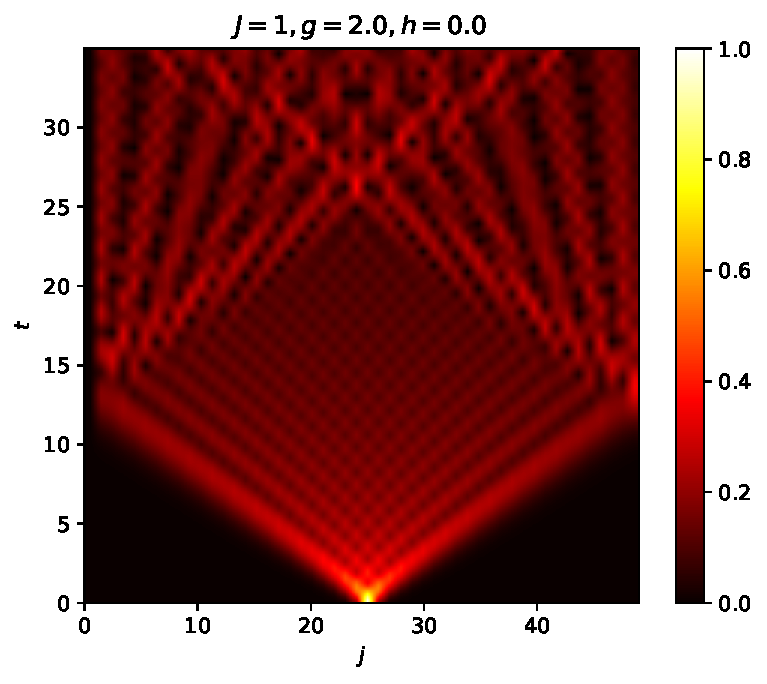
\includegraphics[width=0.49\textwidth]{day2_correlation_g=2.0_L=50_h=0.0.pdf}
    \caption{Time evolution of the correlations of the Ising model with different system parameters.}
\end{figure}

% ----
% \begin{figure}[htbp]
%     \centering
%     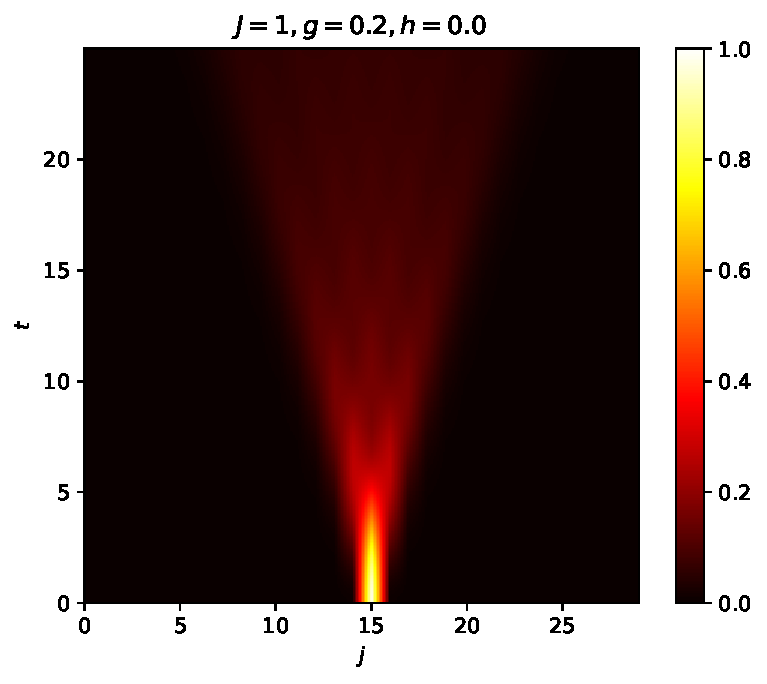
\includegraphics[width=0.7\textwidth]{day2_correlation_g=0.2_L=30_h=0.0.pdf}
%     \caption{}
% \end{figure}

% \begin{figure}[htbp]
%     \centering
%     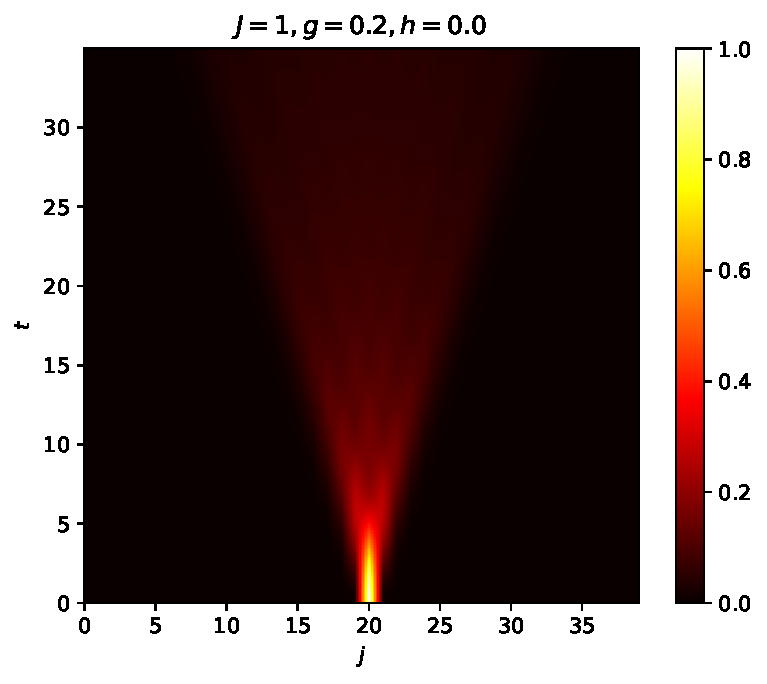
\includegraphics[width=0.7\textwidth]{day2_correlation_g=0.2_L=40_h=0.0.pdf}
%     \caption{}
% \end{figure}

% not generated yet
% \begin{figure}[htbp]
%     \centering
%     \includegraphics[width=0.7\textwidth]{day2_correlation_g=0.2_L=50_h=0.0.pdf}
%     \caption{}
% \end{figure}



% \begin{figure}[htbp]
%     \centering
%     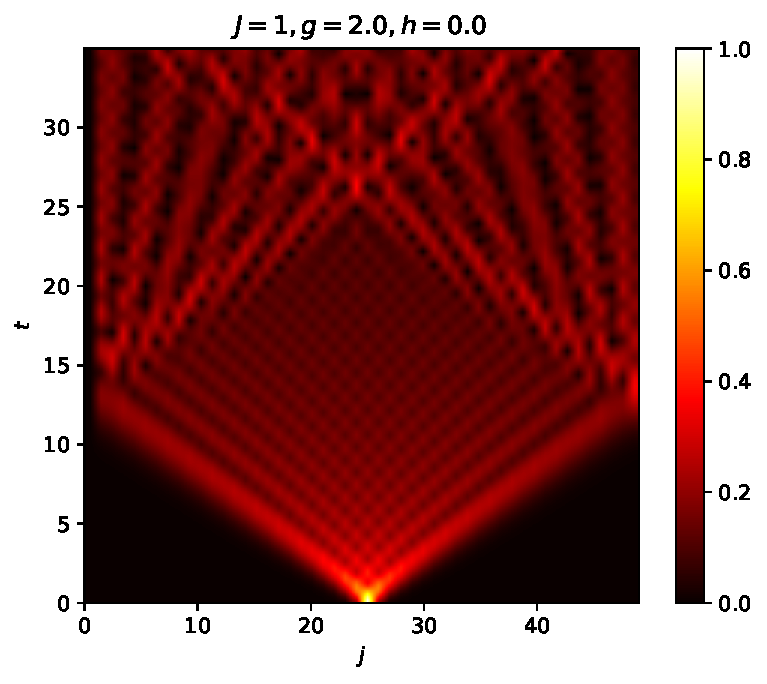
\includegraphics[width=0.7\textwidth]{day2_correlation_g=2.0_L=50_h=0.0.pdf}
%     \caption{}
% \end{figure}


% \begin{figure}[htbp]
%     \centering
%     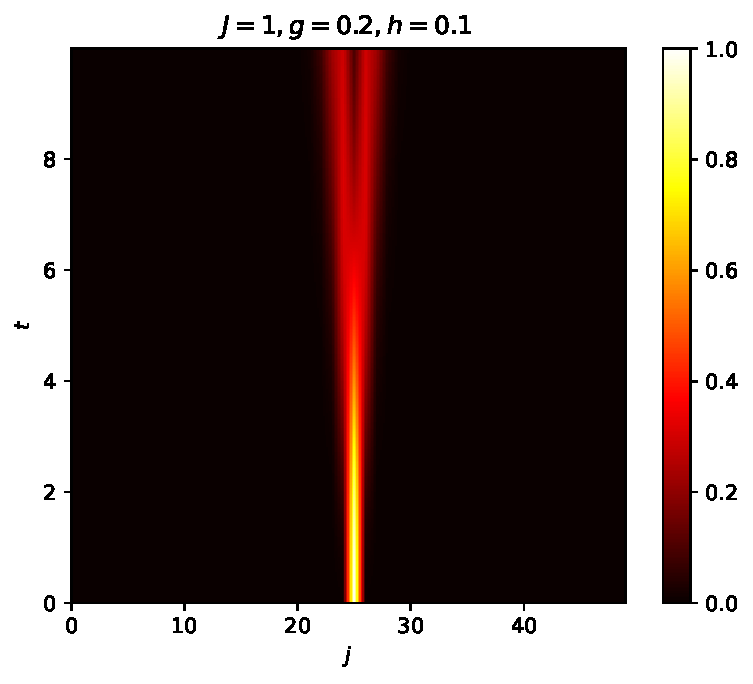
\includegraphics[width=0.7\textwidth]{day2_correlation_g=0.2_L=50_h=0.1.pdf}
%     \caption{}
% \end{figure}



\newpage
\section{Dynamical Spin Structure Factor}
Lastly we want to consider the spectrum of the system.
This is an important quantity, especially with respect to experimental verification, since it can be measured in an experiment.

The spectrum is being obtained by the Fourier transform of the correlation.

First, we are going to neglect the longitudinal field by setting $h=0$.
In this case, we expect a gapless spectrum at the critical point $g=1$, and a gap developing, as we go further away.

In the paramagnetic phase $g=\num{2}$ we can recognize a cosine shaped plot, that has in fact a gap at $k=0$.
Therefore our results are consistent with our expectation.

In the ferromagnetic phase $g=\num{0.2}$ we obtain a smeared out line, with the highest uncertainty at $k=0$.
Physically speaking, we now have 2 domain walls, that can propagate freely in the system.
This causes the obtained spectrum.

\begin{figure}[htbp]
    \centering
    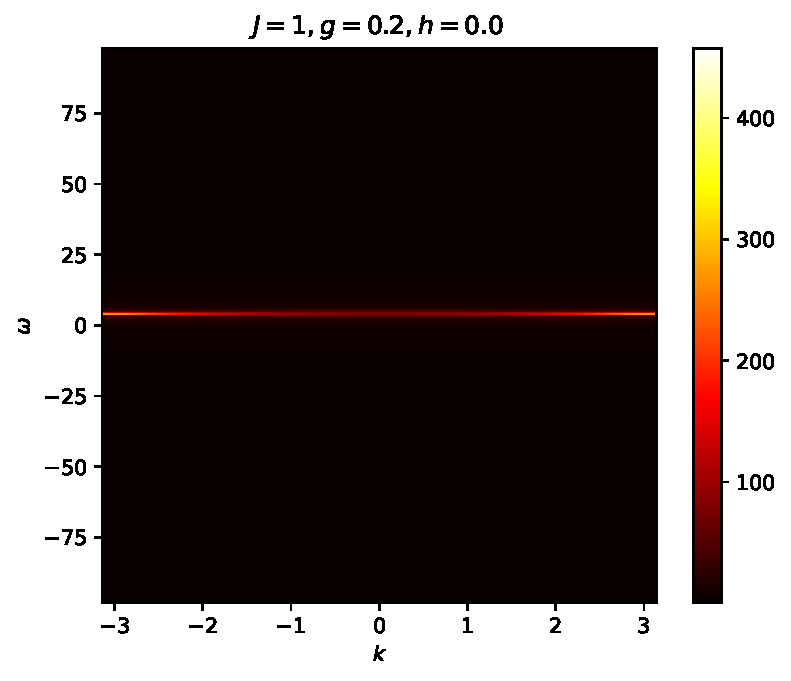
\includegraphics[width=0.49\textwidth]{day2_spectrum_L=40_g=0.2_h=0.0.pdf}
    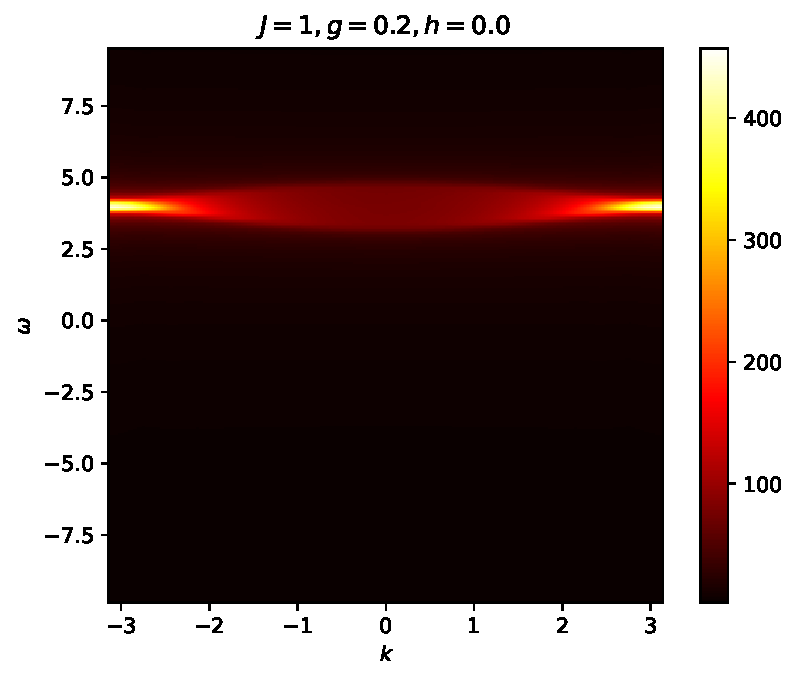
\includegraphics[width=0.49\textwidth]{day2_spectrum_L=40_g=0.2_h=0.0_zoom.pdf}
    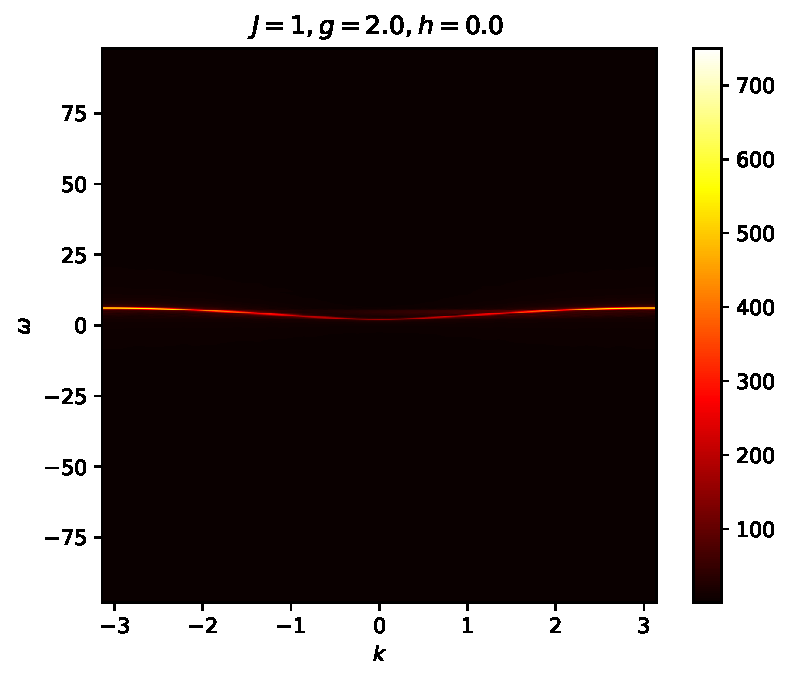
\includegraphics[width=0.49\textwidth]{day2_spectrum_L=50_g=2.0_h=0.0.pdf}
    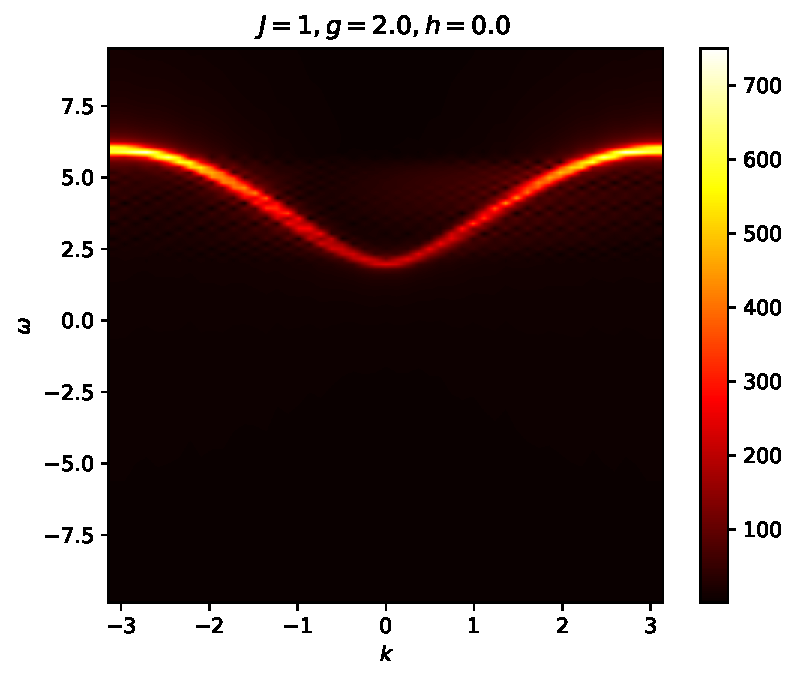
\includegraphics[width=0.49\textwidth]{day2_spectrum_L=50_g=2.0_h=0.0_zoom.pdf}
    \caption{Spectrum of the Ising model for two different regimes $g=\num{0.2}$ and $g=\num{2}$. All plots horizontal next to each other show the same data, just with the right one being zoomed in a little bit.}
\end{figure}


% \begin{figure}[htbp]
%     \centering
%     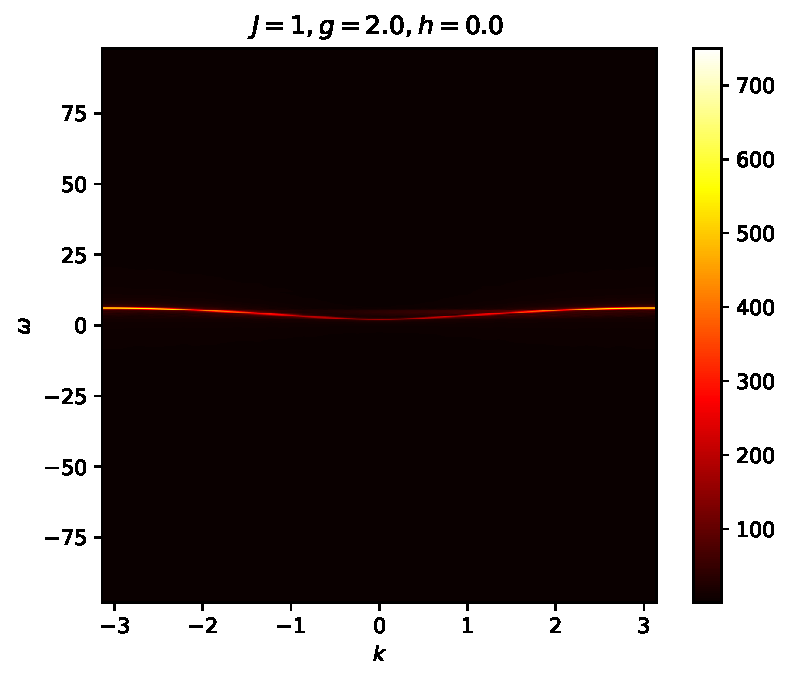
\includegraphics[width=0.49\textwidth]{day2_spectrum_L=50_g=2.0_h=0.0.pdf}
%     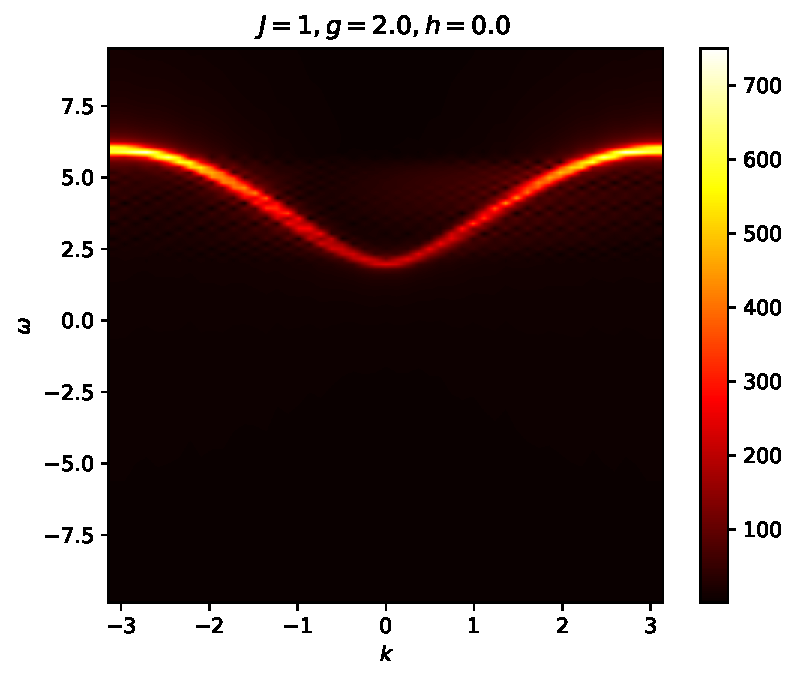
\includegraphics[width=0.49\textwidth]{day2_spectrum_L=50_g=2.0_h=0.0_zoom.pdf}
%     \caption{with $h\neq 0$}
% \end{figure}


\newpage
If we now additionally consider a small longitudinal field $h=\num{0.1}$, we can think of it as an confining potential.
We therefore expect to trap the domain walls (those excitations are also called kinks).

Since we now have an longitudinal field, the spins have a preferred direction.
If the domain walls move apart from each other, it requires an additional energy.
Therefore the excitation with the lowest energy is just a single spin opposite of the favored direction.
We can think of it like a bound state of pairs of kinks.
Those bound states can be seen in the multiple excitations in the spectrum in \autoref{fig:spectrum-h}.

\begin{figure}[htbp]
    \centering
    % 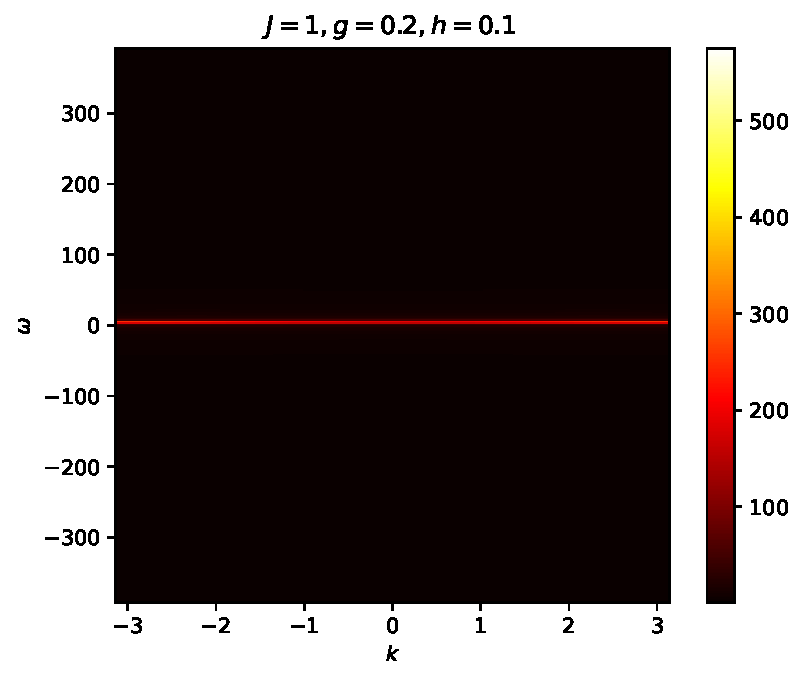
\includegraphics[width=0.49\textwidth]{day2_spectrum_L=50_g=0.2_h=0.1.pdf}
    % 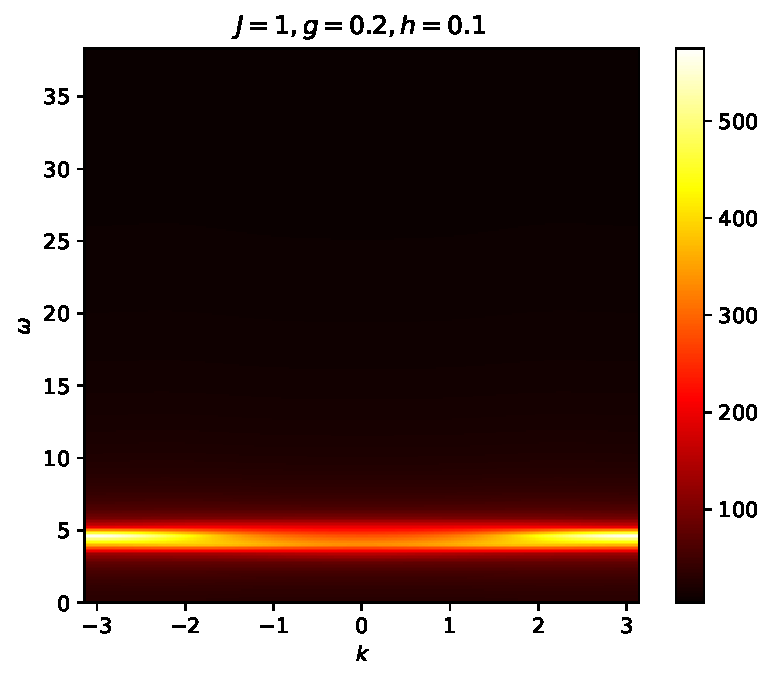
\includegraphics[width=0.49\textwidth]{day2_spectrum_L=50_g=0.2_h=0.1_zoom.pdf}
    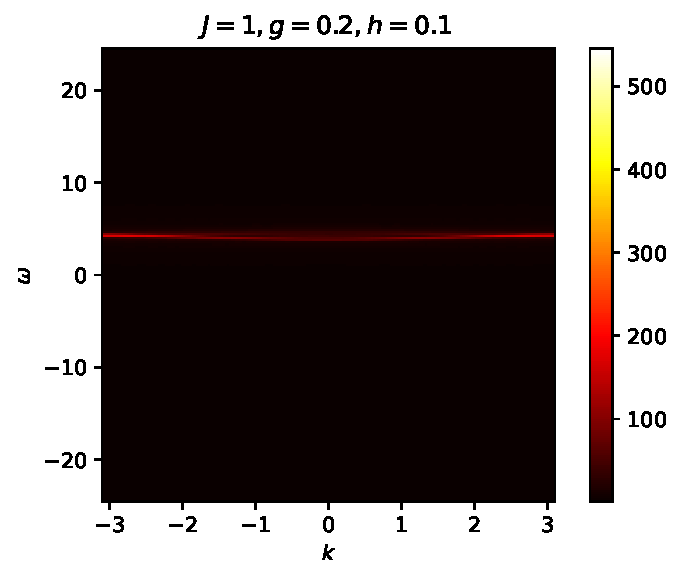
\includegraphics[width=0.49\textwidth]{day2_spectrum_L=81_g=0.2_h=0.1.pdf}
    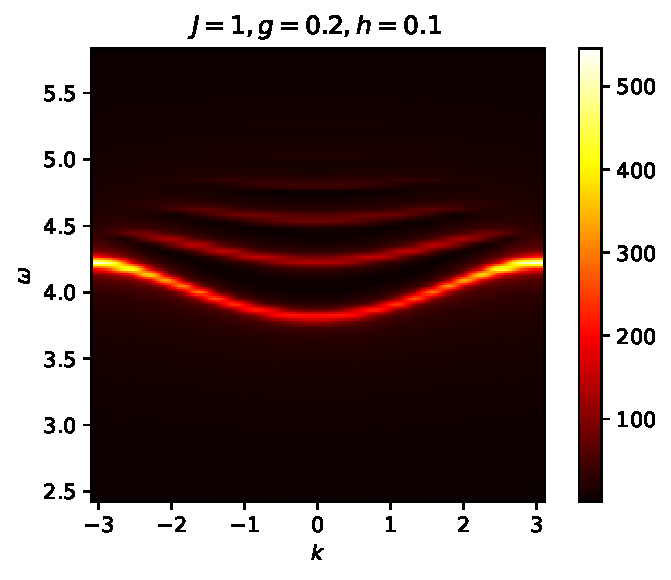
\includegraphics[width=0.49\textwidth]{day2_spectrum_L=81_g=0.2_h=0.1_zoom.pdf}
    \label{fig:spectrum-h}
    \caption{Spectrum of the Ising model with an additional field in $z$ direction ($h=\num{0.1}$). Both plots show the same data, just with the right one being zoomed in a little bit.}
\end{figure}

\newpage
\subsection{Comparison with the Roots of the Airy-function}
In the last part we want to compare the maxima of our structure factor with the negative roots of the Airy function.
This is sensible, since those negative roots are the solution of the corresponding Schrödinger equation~\cite{anleitung}.

In order to compare our results, we use the following relation, given in the solution
\begin{equation}
    m_j = 2\cdot m_0 + c \cdot z_j \label{eq:airy-scale}
\end{equation}
where $m_0$ and $c$ are constants and $z_j$ are the negative roots of the Airy-function $Ai(-z_j) = 0$.

Our results can be seen in \autoref{fig:airy}.
If our simulation were in perfect unison with the theory, the maxima of the blue curve would be exactly at the red marks.
As one can see, this is pretty much the case for the first 4 maxima, then our simulation starts to differ from the expectation.
\begin{figure}[htbp]
    \centering
    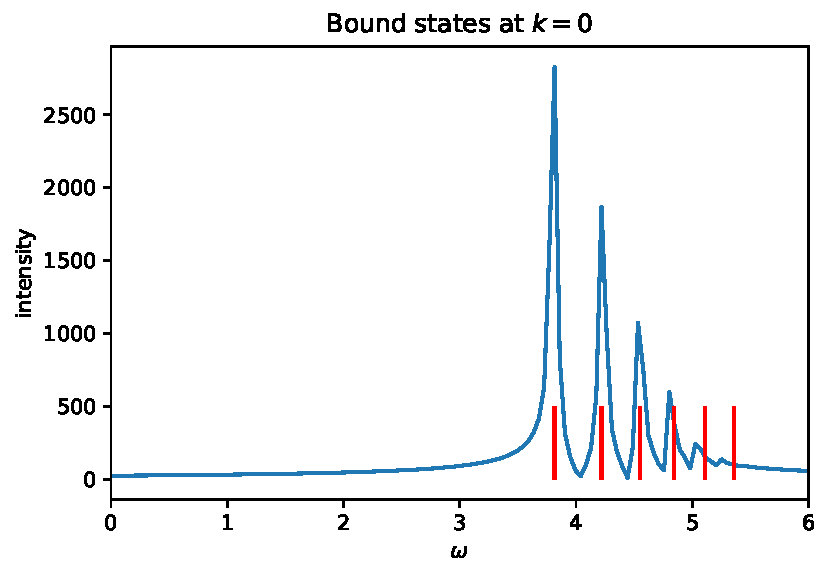
\includegraphics[width=0.7\textwidth]{day2_airy_peaks.pdf}
    \label{fig:airy}
    \caption{Comparison of the structure factor with the theoretical expectation. The horizontal red lines mark the negative roots of the Airy function scaled according to \eqref{eq:airy-scale}.}
\end{figure}
